\chapter{Projekt gry}
\thispagestyle{firststyle}

\section{Ogólna koncepcja gry}

    Jak wspomniano w poprzednim rozdziale, jedna z trudności obserwowanych u osób z zaburzeniami ze spektrum autyzmu dotyczy zdolności rozumienia języka (por. \ref{subsection:rozumienie}).
    Celem opisywanej gry jest wspomaganie ćwiczenia tej umiejętności.
    Postanowiono skoncentrować się na~rozumieniu języka pisanego, ponieważ u osób z autyzmem obserwuje się efektywniejsze przetwarzanie informacji dostarczanych za pomocą modalności wzrokowej w porównaniu do~modalności słuchowej (\cite{quill1997instructional}).
    Zamierzeniem było stworzenie warunków do łatwiejszego skupienia uwagi na ćwiczeniu kompetencji rozumienia języka.
    
    Zastosowanie medium, jakim jest program komputerowy, wynikało z pozytywnego nastawienia do technologii komputerowych, często obserwowanego u osób z autyzmem, a także możliwości dostarczenia użytkownikowi natychmiastowej informacji zwrotnej oraz monitorowania osiąganych postępów i dostosowania zadań do indywidualnych potrzeb użytkowników (por. \ref{subsection:ict}).
    
    Zaprojektowanie aplikacji w formie gry poważnej służyć miało zwiększeniu zaangażowania oraz motywacji użytkowników.
    Aby zachęcić graczy do doskonalenia ćwiczonych umiejętności wprowadzono system punktów zdobywanych za prawidłowe wykonanie poleceń.
    Kolejne podejście do zadania umożliwia osiągnięcie nowego najlepszego wyniku, motywując do~wielokrotnego powtarzania zadań.

\section{Tematyka gry}

    Wybór tematyki miał na celu optymalne połączenie planowanej funkcji edukacyjnej zadań z aspektem rozrywkowym gry.
    Osadzenie gry w realiach detektywistycznych pozwala na~uzasadnione, spójne tematycznie wykorzystanie zadań obejmujących odpowiadanie na pytania w~oparciu o wypowiedź postaci oraz dedukowanie wniosku na podstawie śladów.
    Gracz wcielając się w rolę detektywa rozwiązuje zagadki dotyczące skradzionych przedmiotów.
    Gra zawiera dziesięć spraw (śledztw), z których każda ma jednakową strukturę złożoną z czterech zadań (tab. \ref{table:zadania}).
    
    W warstwie fabularnej w pierwszym zadaniu detektyw notuje szczegóły sprawy zawarte w wypowiedzi klienta.
    Drugie zadanie polega na przeszukaniu miejsca przestępstwa w celu odnalezienia śladów pozostawionych przez sprawcę.
    W trzecim zadaniu detektyw na podstawie odnalezionych poszlak i opisów podejrzanych wnioskuje, kto jest sprawcą.
    W ostatnim zadaniu odzyskuje skradziony przedmiot ukryty przez przestępcę.
    
    \begin{table}
        \begin{tabularx}{\textwidth}{ l X X }
         \hline
         
         \hline
          & \textbf{Treść zadania} & \textbf{Forma zadania} \\
          \hline
         1. & Ustalenie szczegółów sprawy & Dopasowanie odpowiedzi do pytań na~podstawie podanego tekstu \\
         2. & Odszukanie śladów & Wskazywanie obiektów na ilustracji zgodnie z instrukcją \\
         3. & Wywnioskowanie, kto jest sprawcą & Dopasowanie symboli śladów do podanych opisów postaci \\
         4. & Uzyskanie kodu do sejfu ze skradzionym przedmiotem & Odpowiedź na pytania jednokrotnego wyboru \\
         \hline
         
         \hline
        \end{tabularx}
        \caption{Treść i forma zadań}
        \label{table:zadania}
    \end{table}

\section{Projekt ćwiczeń}

    Projekt ćwiczeń uwzględnia fakt, że osoby z autyzmem lepiej funkcjonują w znanej strukturze (Flannery i Horner, \cite*{flannery1994relationship}).
    Zadania w grze opierają się na stałym schemacie, który ma~na~celu zaspokajanie potrzeby przewidywalności.
    Jednocześnie treść ćwiczeń zawiera element losowości i może być w dużym stopniu modyfikowana i rozwijana.
    Wprowadzenie zmienności treści służy zwiększeniu efektywności gry jako narzędzia doskonalącego czytanie ze zrozumieniem.
    Taka konstrukcja zadań ma prowadzić do generalizowania ćwiczonej umiejętności, zapobiegając ograniczeniu gry do powtarzania zapamiętanych przykładów.
    
    \subsection{Pierwsze zadanie}
    
    Pierwsze zadanie (ustalenie przez detektywa szczegółów sprawy) polega na przeczytaniu wypowiedzi postaci oraz dopasowaniu podanych odpowiedzi do pytań (tab. \ref{table:zadanie1}).
    Wypowiedź zawiera informacje na temat zaginionego przedmiotu, miejsca i czasu kradzieży oraz dodatkowych szczegółów dotyczących okoliczności zdarzenia.
    W celu zwiększenia poziomu trudności zadania lista odpowiedzi zawiera dodatkowe opcje, niepasujące do żadnego pytania.
    Zarówno pasujące, jak i niepasujące odpowiedzi zawierają fragmenty informacji pojawiających się w~tekście.
    Dzięki temu do wykluczenia nieprawidłowych odpowiedzi niezbędne jest zrozumienie pytania i powiązanie go z właściwą informacją.
    
    Powyższe zadanie wymaga zidentyfikowania typu informacji (np. opisu czasu, opisu miejsca, przyczyny).
    Pytania mają wspomagać zrozumienie struktury tekstu i ujęcie narracji w~spójną całość (\cite{gately2008facilitating}).
    Ponadto z uwagi na większe trudności w rozumieniu treści odnoszącej się do kontekstu społecznego (Brown, Oram-Cardy i Johnson, \cite*{brown2013meta}), związane z typowymi dla ASD deficytami w zakresie interakcji społecznych oraz zaburzeniami rozwoju teorii umysłu (por. \ref{subsubsection:teoriaumyslu}), w zadaniu wykorzystano teksty i pytania dotyczące sytuacji społecznych (np. pytania o motywacje działań postaci).
    
    \begin{table}
        \begin{tabularx}{\textwidth}{ l X X }
          \hline
        
          \hline
          \multicolumn{3}{c}{\textbf{Wypowiedź postaci}} \\
          \hline
          \multicolumn{3}{ >{\hsize=\dimexpr2\hsize+3\tabcolsep+\arrayrulewidth\relax}X }{,,Dzień dobry! Mam na imię Emilia, jestem mamą pięcioletniego Krzysia. W sobotę po~południu byliśmy na placu zabaw. Mój synek huśtał się na huśtawce, a ja siedziałam na ławce i robiłam mu zdjęcia. Nagle Krzyś spadł z huśtawki, a ja pobiegłam mu~pomóc. Zostawiłam aparat fotograficzny na ławce. Na szczęście Krzysiowi nic się nie stało, więc wróciliśmy po aparat, jednak okazało się, że ktoś go ukradł! Proszę odnaleźć złodzieja!''}  \\
          \hline
          & \textbf{Pytanie} & \textbf{Odpowiedź}\\
          \hline
         1. & ,,Co zginęło?'' & ,,aparat fotograficzny'' \\
         2. & ,,Kiedy doszło do kradzieży?'' & ,,w sobotę po południu'' \\
         3. & ,,Gdzie doszło do kradzieży?'' & ,,na placu zabaw'' \\
         4. & ,,Jak ma na imię synek Emilii?'' & ,,Krzyś'' \\
         5. & ,,Ile lat ma synek Emilii?'' & ,,pięć'' \\
         6. & ,,Dlaczego mama pobiegła do synka?'' & ,,bo spadł z huśtawki'' \\
         7. & ,,Gdzie mama położyła aparat?'' & ,,na ławce'' \\
         8. & \emph{niepasująca odpowiedź} & ,,na huśtawce'' \\
         9. & \emph{niepasująca odpowiedź} & ,,bo chciała zrobić mu zdjęcie'' \\
         \hline
         
         \hline
        \end{tabularx}
        \caption{Zadanie pierwsze: przykładowa wypowiedź postaci wraz z pytaniami}
        \label{table:zadanie1}
    \end{table}
    
    \subsection{Drugie zadanie}
    Zadanie drugie w warstwie fabularnej reprezentuje przeszukiwanie miejsca, w którym dokonano kradzieży, w celu odnalezienia śladów pozostawionych przez złodzieja.
    W grze występuje dziesięć różnych miejsc: pokój 1., pokój 2., sklep ze sprzętem elektronicznym, sklep z zabawkami, muzeum, restauracja, sala szkolna, plac zabaw, plaża, ogród.
    Gracz na ilustracji przedstawiającej miejsce przestępstwa wskazuje opisane przez instrukcję obiekty (tab. \ref{table:zadanie2}).
    Po~poprawnym wskazaniu danego obiektu odkrywany jest kolejny symbol poszlaki.
    
    Do wykonania zadania niezbędne jest zintegrowanie poszczególnych informacji zawartych w instrukcjach (np. rodzaj przedmiotu, kolor, rozmiar, położenie) w celu wskazania właściwego obiektu.
    Wprowadzenie zadania polegającego na odnajdywaniu szczegółów na ilustracji ma~również na celu zwiększenie zainteresowania graczy.
    Ponadto treść zadania służy zachowaniu ciągłości tematycznej gry (odnajdywanie poszlak wykorzystywanych w kolejnym zadaniu).
    
    \begin{table}
        \begin{tabularx}{\textwidth}{ l l X }
         \hline
        
         \hline
          & \textbf{Miejsce przestępstwa} & \textbf{Przykładowa instrukcja} \\
          \hline
         1. & Pokój & ,,Zajrzyj za fioletową książkę na drugiej półce od dołu'' \\
         2. & Sklep elektroniczny & ,,Poszukaj za aparatem fotograficznym leżącym na środkowej półce'' \\
         3. & Restauracja & ,,Sprawdź za lewą zasłoną prawego okna'' \\
         4. & Plac zabaw & ,,Poszukaj pod drzewem koło latarni z lewej strony'' \\
         \hline
         
         \hline
        \end{tabularx}
        \caption{Zadanie drugie: przykładowe instrukcje}
        \label{table:zadanie2}
    \end{table}
    
    \subsection{Trzecie zadanie}
    W trzecim zadaniu (wywnioskowanie, kto z podejrzanych jest sprawcą) na podstawie opisów podejrzanych oraz symboli odnalezionych śladów należy wskazać osobę, z którą związana jest największa liczba poszlak.
    Każde zdanie składające się na opis podejrzanego dotyczy jednej cechy osoby (np. wykonywanego zawodu lub zainteresowań) i odpowiada jednemu symbolowi poszlaki (tab. \ref{table:zadanie3}).
    
    Zadanie składa się dwóch komponentów: zidentyfikowania cech odpowiadających każdemu z symboli śladów oraz odnalezienia opisu zawierającego wszystkie cechy.
    Opisy cech nie zawierają wyrażonych wprost nazw przedmiotów stanowiących poszlaki, odnosząc się przykładowo do nadrzędnej kategorii semantycznej (np. cecha: ,,Bardzo lubi owoce'', poszlaka: skórka od banana).
    W ten sposób starano się uniknąć ograniczenia zadania do dopasowania pojedynczych słów do obrazków.
    
    \begin{table}
        \begin{tabularx}{\textwidth}{ l X X }
         \hline
        
         \hline
          & \textbf{Cecha osoby podejrzanej} & \textbf{Powiązana poszlaka} \\
          \hline
         1. & ,,Pracuje w zakładzie samochodowym'' & Klucz płaski \\
         2. & ,,Jest krawcem''/,,Jest krawcową'' & Igła z nitką \\
         3. & ,,Lubi słodycze'' & Ciastko \\
         4. & ,,Ma słaby wzrok'' & Okulary \\
         \hline
         
         \hline
        \end{tabularx}
        \caption{Zadanie trzecie: przykładowe fragmenty opisów podejrzanych}
        \label{table:zadanie3}
    \end{table}
    
    \subsection{Czwarte zadanie}
    Czwarte zadanie w warstwie fabularnej polega na uzyskaniu kodu do sejfu ze skradzionym przedmiotem.
    Kod składa się z numerów poprawnych odpowiedzi kolejnych pytań.
    Zadanie zawiera trzy typy pytań jednokrotnego wyboru z czterema możliwymi odpowiedziami (tab. \ref{table:zadanie4}).
    Pytania pierwszego typu wymagają wskazania słowa niepasującego (należącego do innej kategorii semantycznej) do pozostałych (np. nazwy pojazdu wśród nazw mebli).
    Drugi typ pytań stanowią zdania z luką, w których należy uzupełnić zdanie wybierając wyrażenie spójne z treścią zdania.
    Pytania trzeciego typu również zawierają zadania z luką, jednak wymagają wskazania odpowiedzi niepasującej do kontekstu zdania.
    
    Powyższe zadanie ma na celu ćwiczenie umiejętności generalizowania znaczeń pojedynczych słów i odnoszenia ich do kontekstu semantycznego.
    Deficyty w zakresie tej kompetencji wiążą się z obserwowaną u osób z ASD tendencją do koncentrowania się na szczegółach, opisywaną przez teorię słabej centralnej koherencji (por. \ref{subsubsection:teoriakoherencji}).
    Ponadto zdania z luką obejmują przykłady dotyczące sfery emocji (przypisywanie emocji do podanej sytuacji oraz identyfikowanie sytuacji stanowiącej przyczynę podanej emocji), która również stanowi obszar trudności typowy dla zaburzeń ze spektrum autyzmu (Begeer, Koot, Rieffe, Terwogt i Stegge, \cite*{begeer2008emotional}).
    
    \begin{table}
        \begin{tabularx}{\textwidth}{ l X }
         \hline
        
         \hline
            & \textbf{Przykładowe pytanie i odpowiedzi} \\
         \hline
         1. & Które słowo nie pasuje do pozostałych? \\
            & 1) burza 2) wiatr 3) złość 3) chmury \\
         2. & Która odpowiedź pasuje w puste miejsce? \\
            & ,,Marcin był z siebie dumny, bo ... .'' \\
            & 1) zgubił się w lesie 2) pochwalił go tata 3) zapomniał kluczy 4) miał brudne buty \\
         3. & Która odpowiedź nie pasuje w puste miejsce? \\
            & ,,Brat Kasi był ... , bo spóźnił się na pociąg.'' \\
            & 1) niezadowolony 2) zdenerwowany 3) smutny 4) rozbawiony  \\
         \hline
         
         \hline
        \end{tabularx}
        \caption{Zadanie czwarte: przykładowe pytania jednokrotnego wyboru}
        \label{table:zadanie4}
    \end{table}

\section{Projekt interfejsu użytkownika}
    Jednym z założeń projektu gry było stworzenie interfejsu przystępnego dla osób z ASD.
    Wśród zaleceń dotyczących projektowania interfejsu użytkownika dla osób z ASD wymienia się stosowanie łagodnych i stonowanych kolorów, prostych grafik oraz czytelnych krojów pisma (\cite{pavlov2014user}).
    Interfejs powinien posiadać przejrzystą nawigację z jasno wskazanym aktualnym położeniem użytkownika, wizualne wskaźniki czasochłonnych akcji oraz przycisk pomocy.
    Wskazane jest prezentowanie niewielkiej liczby elementów na ekranie, zastosowanie dużych przycisków z ikoną i tekstem oraz dostarczanie użytkownikowi krótkich instrukcji na~każdym etapie interakcji z systemem (\cite{pavlov2014user}).
    
    W aplikacji wykorzystane zostały elementy stylu graficznego Material Design oraz ikony z zestawu Font Awesome.
    Ilustracje do gry wykonano w minimalistycznej estetyce, bazując na prostych geometrycznych kształtach.
    Podczas doboru kolorów unikano barw o wysokim nasyceniu.
    Jako oznaczenie czasochłonnych akcji (np. logowania użytkownika) zastosowano animowaną ikonę.
    W celu oznaczenia postępu gracza w widoku sprawy umieszczono pasek z~czterema ikonami oznaczającymi kolejne zadania i wyróżnieniem ikony aktualnego zadania.
    
    Do każdego zadania zaprojektowano prostą instrukcję, opisującą kolejne czynności, które ma wykonać gracz.
    Każda instrukcja składa się z dwóch lub trzech poleceń wraz z ich graficzną reprezentacją w formie piktogramów (rys. \ref{fig:instrukcja}).
    
    \begin{figure}
        \centering
        \begin{subfigure}{0.5\linewidth}
            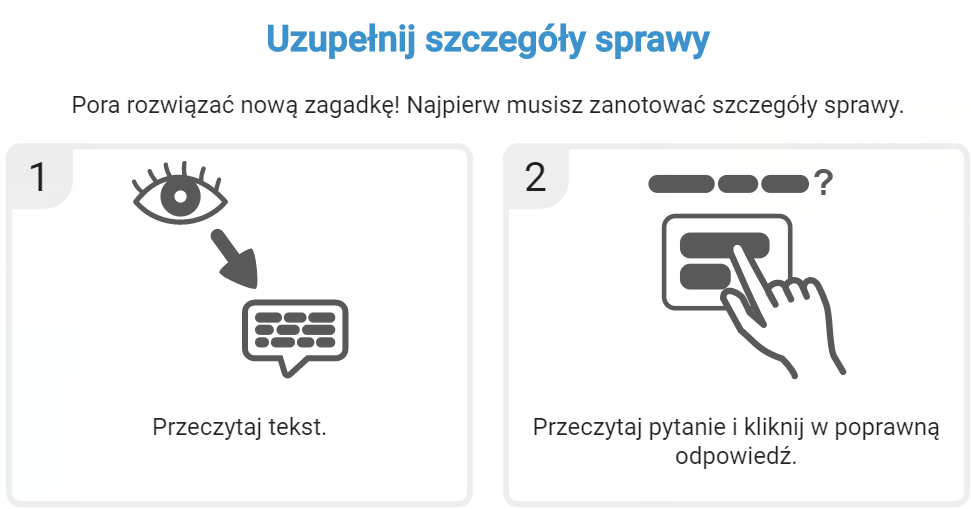
\includegraphics[width=\linewidth]{instrukcja_01}
            \caption{Zadanie pierwsze}
        \end{subfigure}
        \par\bigskip
        \begin{subfigure}{0.5\linewidth}
            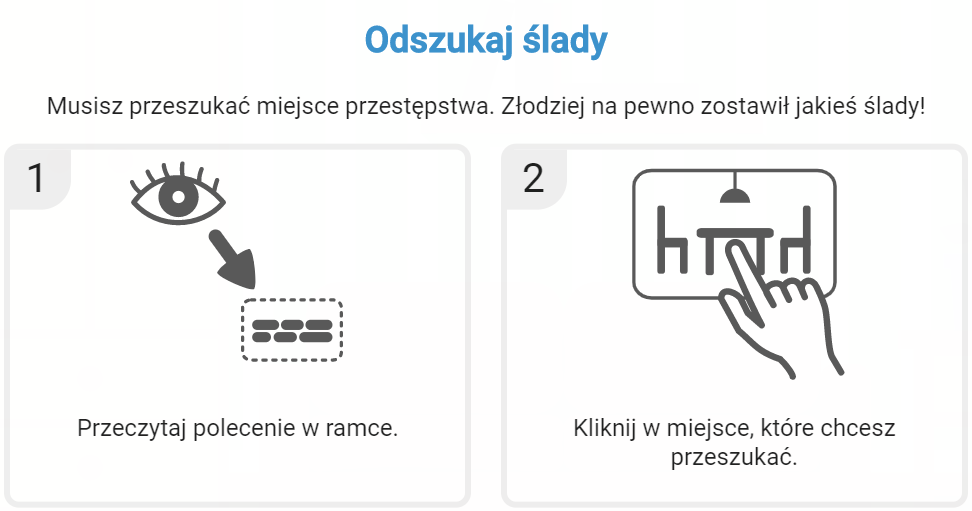
\includegraphics[width=\linewidth]{instrukcja_02}
            \caption{Zadanie drugie}
        \end{subfigure}
        \par\bigskip
        \begin{subfigure}{0.75\linewidth}
            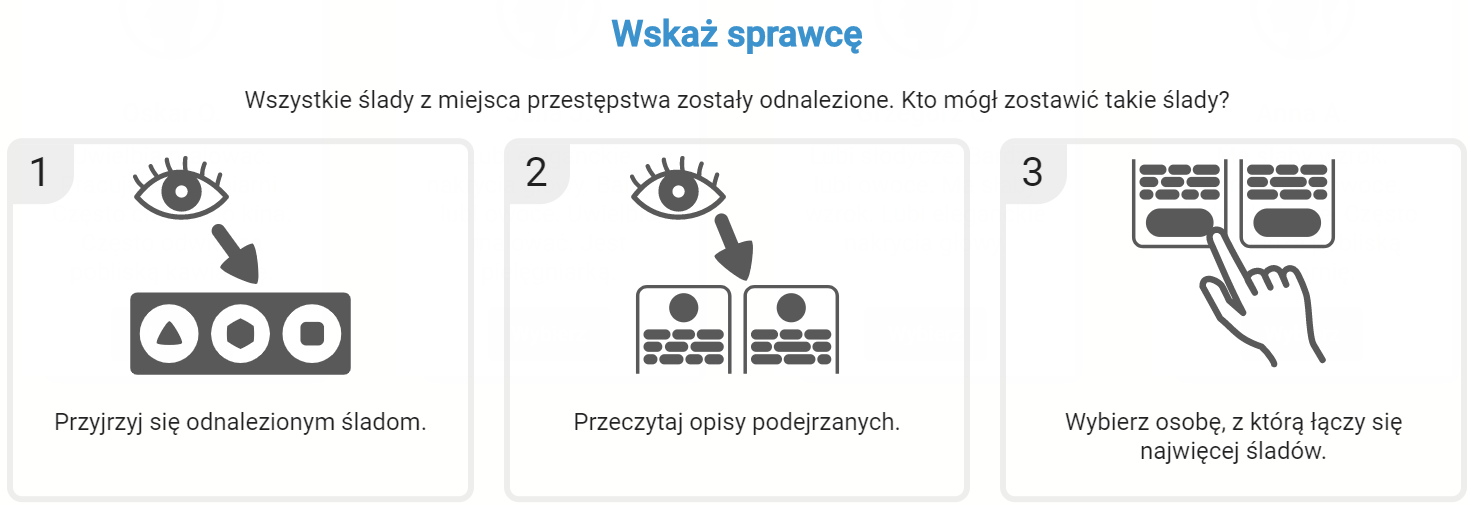
\includegraphics[width=\linewidth]{instrukcja_03}
            \caption{Zadanie trzecie}
        \end{subfigure}
        \par\bigskip
        \begin{subfigure}{0.5\linewidth}
            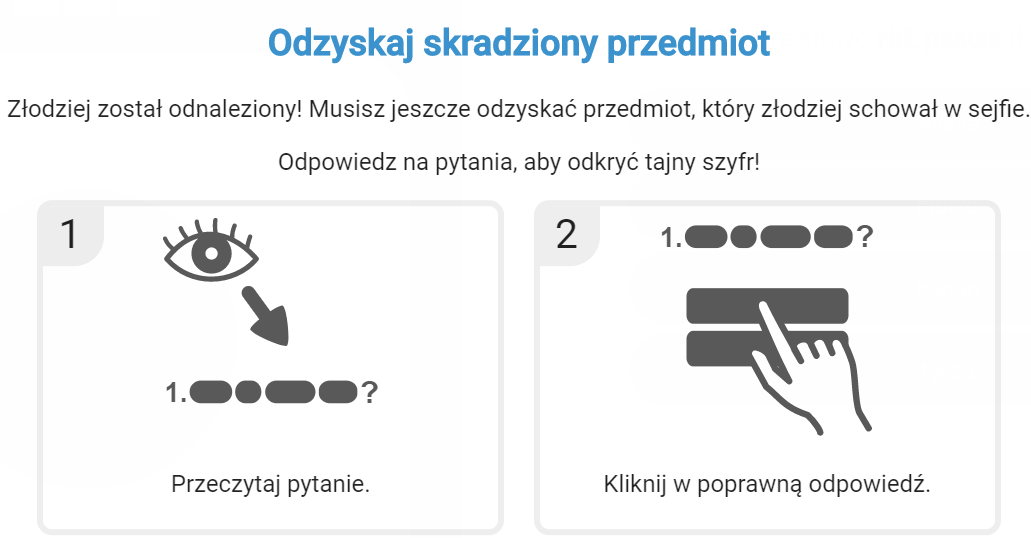
\includegraphics[width=\linewidth]{instrukcja_04}
            \caption{Zadanie czwarte}
        \end{subfigure}
        \caption{Instrukcje do zadań}
        \label{fig:instrukcja}
    \end{figure}
